% !TEX root = ../main.tex

\begin{figure}[t]
\centering
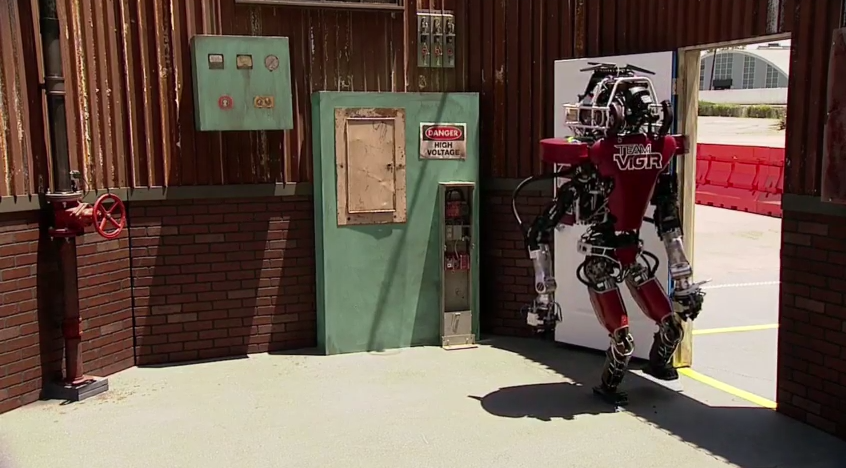
\includegraphics[width=0.99\columnwidth,clip]{./img/atlas_door_finals.png}
\caption{Team ViGIR's Atlas humanoid robot on the first day of the DRC Finals. (Photo credit: DARPA)
}
\label{Fig:AtlasDoorFinals}
\end{figure}

In preparation for the 2015 DARPA Robotics Challenge (DRC) Finals, Team ViGIR, as well as many other teams, developed an approach to high-level robot control \cite{Philipp2013Bsc, Philipp2015Msc}.
However, these approaches relied on experts developing scripted behaviors or, in the case of Team ViGIR, manually designing state machines.
In addition, there was no guarantee that the resulting high-level behavior was correct with respect to the task at hand.
Moreover, many participants observed that such approaches were fragile in practice \cite{DRC-what-happened}.

Motivated by these shortcomings, we present an approach for the automatic generation of software that implements high-level robot behaviors in a provably-correct manner.
This was enabled in part by recent advances in the field of formal methods for robotics.
Specifically, correct-by-construction mission plans can be automatically synthesized from high-level, logic-based specifications [cite ALL the papers].

\begin{myExample}\label{Ex:PickupObject}
	Consider the high-level task: ``Walk to the valve and turn it" (Fig. \ref{Fig:AtlasDoorFinals}).
	This would be an intuitive way to express the task from a non-expert user's point-of-view.
	However, \ldots (not formal, capabilities (a robot with no manipulators wouldn't be able to carry out this task), reaction to failures, etc.)
\end{myExample}

Writing a formal, logic-based specification is a non-trivial task that requires expert knowledge.
In this paper, we automatically generate the logic-based specifications from a higher level, partial, multi-paradigm specification: a description of the system's capabilities, a list of the task's goals, and the task's initial conditions.
Furthermore, most approaches in this field assume that the simple, low-level components that make up the high-level plan will work as expected, i.e., they never fail.
In this paper, we take a first step towards lifting this assumption by formally accounting for the possibility of failure when executing the low-level components.
We achieve this by generalizing the concepts of ``activation" and ``completion" as presented in \cite{Vasu2013ICRA} to deal with a different problem in logic-based synthesis.
While a failure is still a failure and there might be no way to recover, we can still achieve \emph{graceful degradation}.

Ours is an end-to-end approach that starts with an informal specification and results in an executable software implementation of a high-level plan.
We first create a discrete abstraction of the problem and automatically construct a formal task specification in a fragment of Linear Temporal Logic (\textsc{LTL}).
We then synthesize a \emph{reactive} mission plan that is guaranteed to satisfy the formal specification.
Finally, in an effort to bridge the gap between theoretical results and practice, we automatically generate a state machine that instantiates the synthesized plan in software.

In this paper, we present and experimentally validate the proposed approach in the context of a Boston Dynamics Atlas humanoid robot running the software that Team ViGIR developed for the DARPA Robotics Challenge (Fig. \ref{Fig:AtlasDoorFinals}).
However, the concepts apply to different systems.
Finally, we have implemented and open-sourced the proposed approach as a collection of Robot Operating System (ROS) packages.

\subsubsection*{Literature Survey}
\begin{itemize}
	\item Vasu's ``fast-slow" paradigm \cite{Vasu2013ICRA}
	\item Alternatives to LTL and GR(1) Synthesis
	\begin{itemize}
		\item Classic AI planners, STRIPS-type planners
		\item Optimization-based LTL synthesis (Eric Wolff)
		\item \textbf{co-safe LTL} (Lydia Kavraki, Calin Belta, etc.) We \emph{could} have used it as a different formalism and generated FlexBE state machines that way.
		\todo[inline, caption = {Comparison of GR(1) to co-safe LTL}]{Check whether co-safe LTL encodes reactivity w.r.t. adversarial environment (worst case)}
	\end{itemize}
\end{itemize}

The rest of this paper is organized as follows. \ldots

%END